\section{棋盘覆盖问题}

\subsection*{\noindent{问题描述}}
设 $n=2^k\,(k\geqslant0)$。在一个 $n×n$ 个方格组成的棋盘中,恰有 1 个方格与其他方格不同,称该方格为特
殊方格。显然,特殊方格在棋盘中可能出现的位置有 $4^k$ 种,因而有 $n^2$ 种不同的棋盘,下图
所示是 $k=2,\,n=4$ 时 16 种棋盘中的一个。
\begin{figure}[htbp]
    \centering
    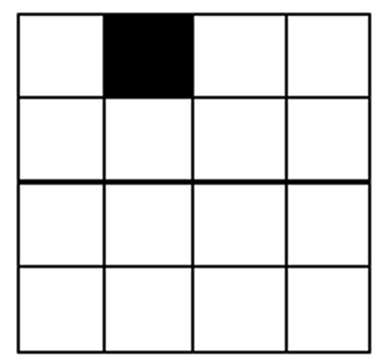
\includegraphics[width=4cm, height=4cm]{figure/chesstable.png}
  \end{figure} 
棋盘覆盖问题要求用下图所示的 4 种不同形状的 $L$ 型骨牌覆盖给定棋盘上除特殊方格以外的所有方格,
且任何 2 个 $L$ 型骨牌不得重叠覆盖。

\begin{figure}[htbp]
  \centering
  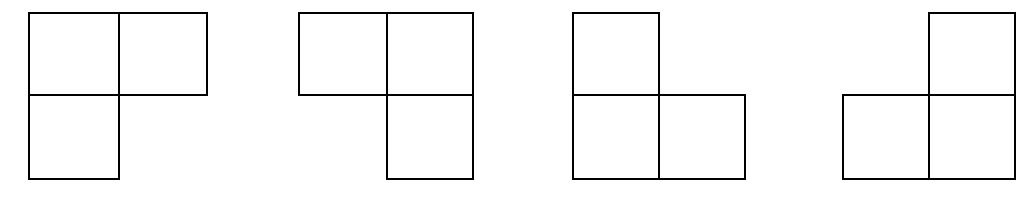
\includegraphics[width=8cm, height=1.5cm]{figure/chesstable2.png}
\end{figure} 

易知,在任何一个 $n×n$ 的棋盘中,用到的 $L$ 型骨牌个数恰为 $(n^2-1)/3$。
若给定棋盘大小 $k>1,\,n=2^k$,请设计一个算法实现棋盘的一种覆盖。

\subsection*{\noindent{问题分析}}
采用分治的思想,将棋盘分割成 4 个 $2^{k-1}×2^{k-1}$ 的子棋盘,对无特殊方格的 3 个子棋盘,
在靠近中心的位置上各添一个特殊方格,使其转化为特殊棋盘。再对 4 个含特殊方格的子棋盘进行同样处理。

算法的时间复杂度递推式为:
\[ T(n) = \left\{
\begin{array}{lr}
4T(n/2)+O(1) & (n>1) \\
O(1) & (n=1)
\end{array} \right. \]

\newpage

\subsection*{\noindent{实验程序代码}}
\begin{code}
    \lstinputlisting[language=C]{code/exp1.cpp}
\end{code}

\subsection*{运行结果}

\begin{figure}[htbp]
    \centering
    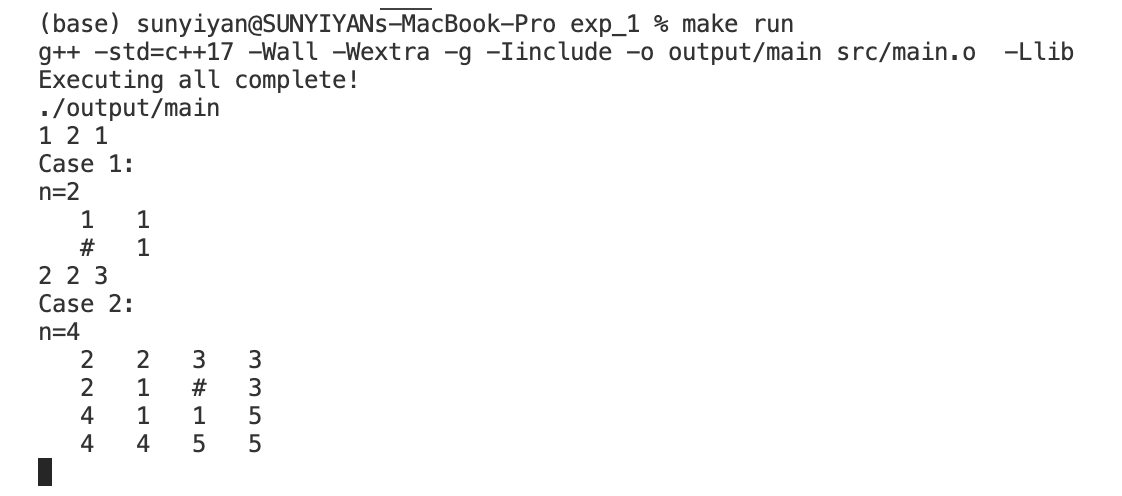
\includegraphics[height=5cm]{figure/run_time_1.png}
    \caption*{数字形式输出棋盘覆盖}
  \end{figure} 

\subsection*{\noindent{实验中遇见的问题}}
本次实验参考了教科书上有例程,太久不写C++,一些语言细节已经记不清,导致在设置二维数组的时候,忘记不能设置固定的空间,而要动态地根据数据规模来申请空间。同时过程中发现使用C++来绘制多色棋盘界面非常困难,由于时间关系并没有继续做下去。
\newpage



\section{矩阵连乘问题}

\subsection*{\noindent{问题描述}}
给定 $n$ 个矩阵 $A_1,A_2,…,A_n$ ,其中,$A_i$与 $A_{j+1}$ 是可乘的,$i=1,2,…,n-l$。
你的任务是要确定矩阵连乘的运算次序,使计算这 $n$ 个矩阵的连乘积 $A_{1}A_{2}…A_{n}$ 时总的元素乘法次数达到最少。

例如: $3$ 个矩阵 $A_1,A_2,A_3$ ,阶分别为 $10×100 100×5 5×50$ ,计算连乘积 $A_1*A_2*A_3$ 时按$(A_1*A_2)*A_3$所需的元素乘法次数达到最少,为 $7500$ 次。


\subsection*{\noindent{问题分析}}
由题意知可将矩阵 $A_1$ 表示为 $p*q$ ,矩阵 $A_2$ 表示为 $q*t$ ,则矩阵 $A_1*A_2$ 所需乘法次数为 $p*q*t$ 。
设$f[L,R]$代表所有将$[L,R]$进行完全加括号得到最终结果的方式的集合,所以$f[L,R]$的值同时也等于该集合的乘法数量最少次数将$f[L,R]$划分子集,其子集有
\begin{enumerate}
    \item $f[L,L]$ 的集合,最少次数为 $f[L + 1,R]+p[L - 1] * p[L] * p[R]$
    \item  $f[L,L + 1]$的集合,最少次数为 $f[L,L + 1] + p[L - 1] * p[L + 1] * p[R] + f[L + 2,R]$
    \item $cf[L,L + 2]$ 的集合,最少次数为 $f[L,L + 2] + p[L - 1] * p[L + 2] * p[R] + f[L + 3,R]$
    \item \dots
    \item $f[L,k]$ 的集合,最少次数为 $f[L][k] + p[L - 1] * p[k] * p[R] + f[k + 1][R]$,其中 $k$ 属于 $[L + 1,R]$
\end{enumerate}
所以动态方程为
\[ f[i][j] = \left\{
\begin{array}{lr}
0 & (i=j) \\
\displaystyle\min_{i\leqslant k<j}\{f[i][k]+f[k+1][j]+p_{i-1}p_kp_j\} & (i\neq j)
\end{array} \right. \]
\newpage

\subsection*{\noindent{实验程序代码}}


\begin{code}
    \lstinputlisting[language=C]{code/exp2.cpp}
\end{code}

\subsection*{运行结果}

\begin{figure}[htbp]
    \centering
    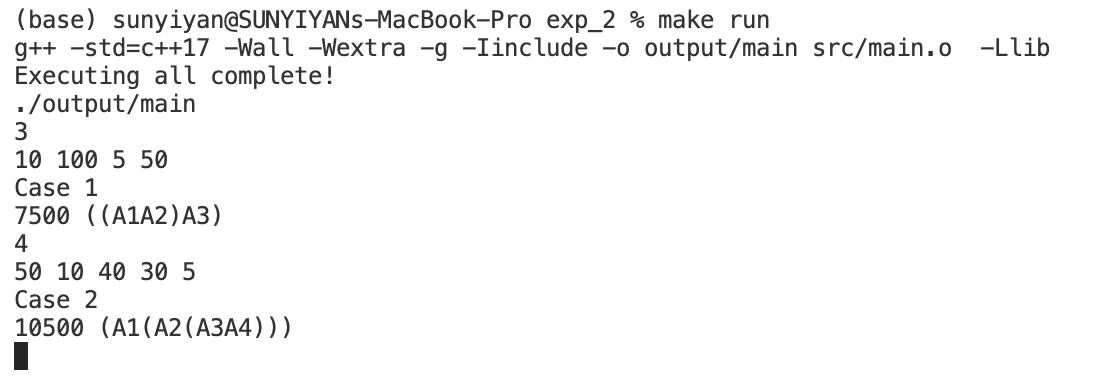
\includegraphics[height=5cm]{figure/run_time_2.png}
  \end{figure} 

\subsection*{\noindent{实验中遇见的问题}}
矩阵连乘积计算次序问题的最优解包含着其子问题的最优解,这也是动态规划题的特征性质,遇见这一类问题解决的关键问题在于根据所给条件找出状态转移方程。

\newpage

\section{最长公共子序列问题}

\subsection*{\noindent{问题描述}}
序列 $Z=<B,\,C,\,D,\,B>$ 是序列 $X=<A,\,B,\,C,\,B,\,D,\,A,\,B>$ 的子序列,相应的递增下标序列为 $<2,\,3,\,5,\,7>$。


一般地,给定一个序列 $X=<x_1,\,x_2,\dots,\,x_m>$,则另一个序列 $Z=<z_1,\,z_2,\dots,\,z_k>$ 是 $X$ 的子序列,
是指存在一个严格递增的下标序列 $<i_1,\,i_2,\dots,\,i_k>$ 使得对于所有 $j=1,\,2,\dots,\,k$ 使 $Z$ 中第 $j$ 个元素 $z_j$ 与 $X$ 中第 $i_j$ 个元素相同。


给定 2 个序列 $X$ 和 $Y$,当另一序列 $Z$ 既是 $X$ 的子序列又是 $Y$ 的子序列时,称 $Z$ 是序列 $X$ 和 $Y$ 的公共子序列。
请给定 2 个序列 $X$、$Y$,并求 $X$ 和 $Y$ 的最长公共子序列 $Z$。


\subsection*{\noindent{问题分析}}
要到 $X$ 和 $Y$中最长的公共子序列,首先需要考虑 $X$ 的最后一个元素和 $Y$ 的最后一个元素。
\begin{enumerate}
    \item 如果 $x_n=y_m$ ,即 $X$ 的最后一个元素与 $Y$ 的最后一个元素相同,这说明该元素位于公共子序列中,因此$LCS(X_{n-1},Y_{m-1})$ 是原问题的一个子问题。
    \item  如果$x_n != y_m$,产生了两个子问题:$LCS(X_{n-1},Y_m)$ 和 $LCS(X_n,Y_{m-1})$。因为序列$X$ 和 序列$Y$ 的最后一个元素不相等,那说明最后一个元素不是最长公共子序列中的元素。所以$LCS(X,Y)=\max({LCS(X_{n-1},Y_m),LCS(X_n,Y_{m-1})})$
\end{enumerate}

动态方程为:
\[ c[i][j] = \left\{
\begin{array}{ll}
0 & (i=0\text{ 或 }j=0) \\
c[i-1][j-1]+1 & (i,\,j>0\text{ 且 }x_i=y_j) \\
\max\{c[i][j-1],\,c[i-1][j]\} & (i,\,j>0\text{ 且 }x_i\neq y_j)
\end{array} \right. \] 

\newpage

\subsection*{\noindent{实验程序代码}}


\begin{code}
    \lstinputlisting[language=C]{code/exp3.cpp}
\end{code}

\subsection*{\noindent{运行结果}}

\begin{figure}[htbp]
    \centering
    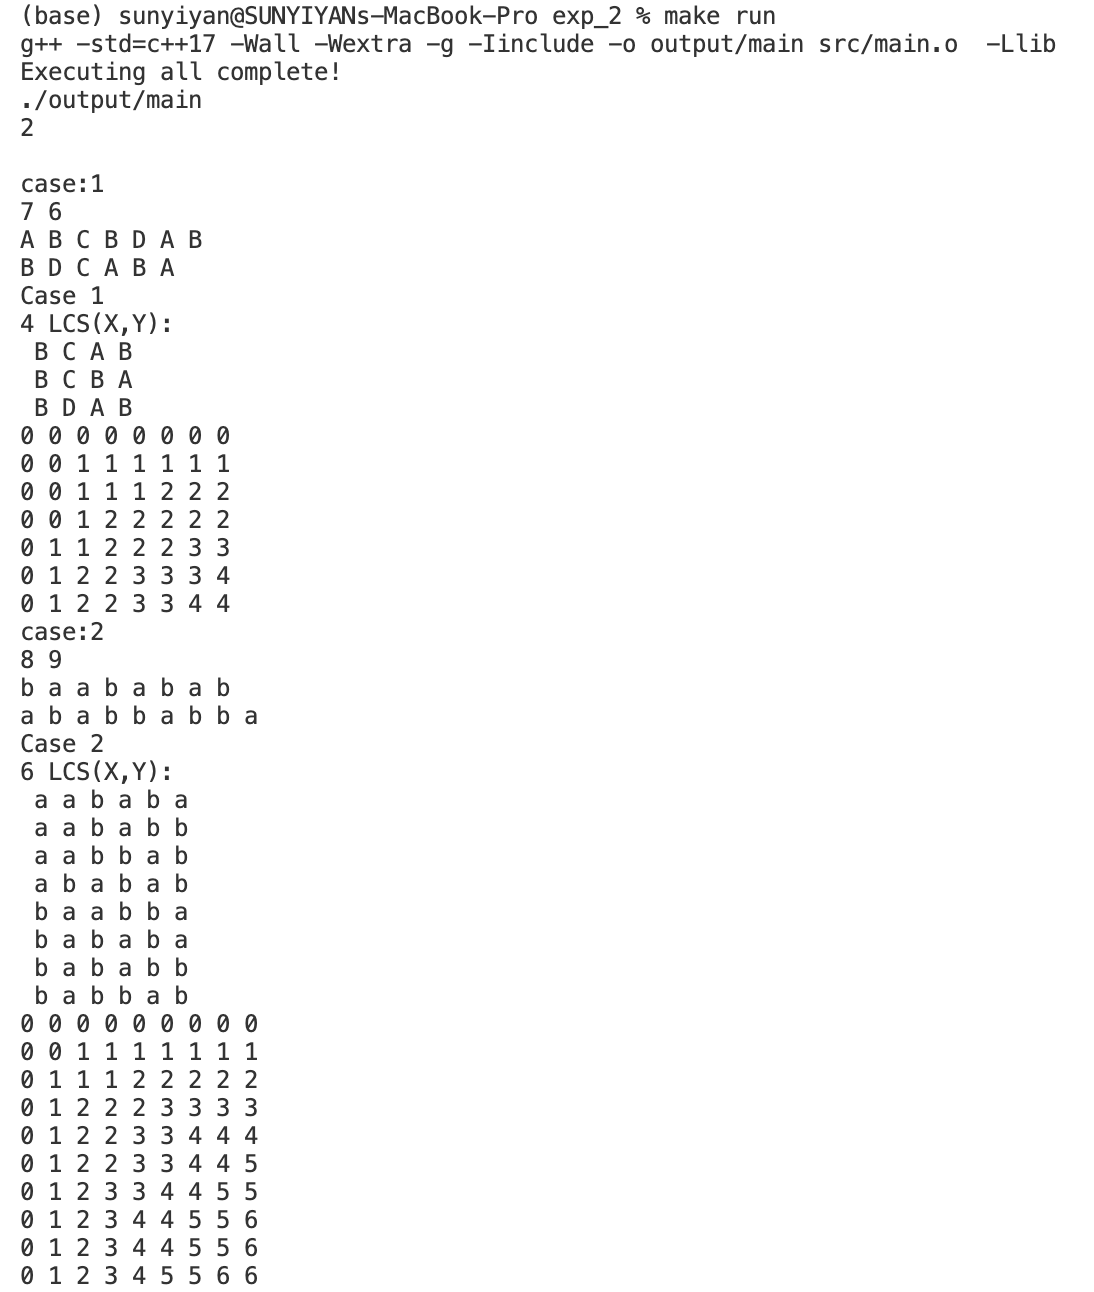
\includegraphics[height=18cm]{figure/run_time_3.png}
  \end{figure} 

\subsection*{\noindent{实验中遇见的问题}}
在输出最长公共子序列的长度的基础上,输出一个最长公共子序列并不难,但是输出全部的最长公共子序列变得困难起来,涉及一个对动态规划过程的回溯,需要自定义状态值线索表来保存状态才能实现目标。


\newpage

